\chapter{کار‌های مشابه}
\section{مقدمه}
در این فصل هدف ما بررسی کارهای مشابه است تا بتوان از آنها در روند بهبود پروژه کمک گرفت. همچنین با توجه به نتایج و ارزیابی پروژه‌های دیگر می‌توان بستری فراهم کرد تا نتیجه پروژه را با دیگر کارهای مشابه مقایسه کرد.
\\
به صورت کلی پروژه‌هایی با هدف کنترل پهپاد با ژست دست در 3 دسته قرار می‌گیرند.
\begin{itemize}
    \item کنترل پهپاد با کمک بینایی ماشین که شامل شبکه‌هایی برای پردازش تصویر است. 
    \item کنترل پهپاد با دستکش‌های سنسور دار از جمله سنسور \lr{IMU} که نیازمند سخت‌افزار خاص برای پیدا کردن موقعیت نقاط کلیدی دست است. با استفاده از یک شبکه عصبی و موقعیت این نقاط می‌توان ژست دست را تشخیص داد. مانند پروژه‌های  \cite{yoo2022motion} و \cite{ma2017hand}.
    \item با کمک دستگاه کنترل‌کننده حرکت جهشی\LTRfootnote{Leap Motion Controller} که با ردیابی دست، ویژگی‌های آن از جمله موقعیت کف دست و انگشتان، جهت دست و انگشتان، طول و عرض انگشتان، موقعیت مفصل و استخوان‌ها را با دقت بالا اندازه‌گیری کرده و با کمک شبکه‌های عصبی ژست دست تشخیص داده میشود. پروژه‌ی
    \cite{hu2020deep} و \cite{sarkar2016gesture} نمونه‌ای از این جمله پروژه‌ها هستند. 
\end{itemize}

از بین این موارد پروژه ما مربوط به اولین گزینه است که تنها سخت‌افزار مورد نیاز به جز پهپاد دوربین نصب شده روی آن است. 
پروژه‌های مشابه با کار ما که با کمک پردازش تصویر پهپاد را کنترل می‌‌کنند به ۳ دسته کلی تفکیک می‌شوند.
\begin{enumerate}
    \item استخراج ویژگی‌های تصویر در هر فریم که با توجه به نیاز‌های مسئله می‌تواند متفاوت باشد، و پیش‌بینی ژست دست براساس آن ویژگی‌ها.
    \item تشخیص دست\LTRfootnote{Hand Detection} ‌برای پیدا کردن موقعیت دست در هر فریم تصویر و ورودی پیکسل‌های \lr{RGB} آن به مدل و در نهایت کلاس‌بندی ژست دست.
    \item استخراج نقاط کلیدی\LTRfootnote{Key Point}  دست در تصویر و ورودی آنها به مدل برای کلاس‌بندی و تشخیص ژست دست.
\end{enumerate}

در ادامه این فصل به بررسی مقالات در این سه زمینه و مقالاتی که بر روی پهباد و پیاده‌سازی مدل‌های هوش مصتوعی تمرکز دارند می‌پردازیم.

\section{مقالات مربوط به ویژگی‌های تصویر}
مقالات به‌کار برده شده در این قسمت بر چگونگی تعیین ژست دست با توجه به تصویر داده‌شده تمرکز دارند. برخی از این مقالات چکونگی ارتباط با پهپاد را نیز پوشش می‌دهند، اما نکته قابل بررسی برای ما چگونگی استخراج ویژگی‌های تصویر و استفاده از آنها برای تعیین ژست دست است.


\subsection{مقاله \lr{Hand Gesture Controlled Drones: An Open Source Library}}
در این پروژه، تمرکز بر پیاده‌سازی یک سیستم کنترل برای هواپیماهای بدون سرنشین با استفاده از حرکات دست است که مشابه رویکرد مورد بحث در مقاله می‌باشد.
هدف اصلی این پروژه استفاده از شبکه‌های عصبی یادگیری عمیق برای تشخیص لحظه‌های حرکات دست پویا برای کنترل پرواز پهپاد 
است. این تشخیص بر اساس ویژگی‌های \lr{Haar} که با توجه به سایه‌ها و رنگ‌های درون تصویر تعیین می‌شوند، انجام می‌شود \cite{natarajan2018hand}.

\subsubsection{روش‌شناسی}
در این پروژه، ابتدا از یک شبکه عصبی برای تشخیص موقعیت دست استفاده می‌شود که به عنوان یک ماژول پیش‌پردازش عمل می‌کند و با دقت بالا موقعیت دست را تشخیص می‌دهد. پس از تشخیص 
موقعیت دست، ویژگی‌های \lr{Haar} از تصویر استخراج می‌شوند. آنها مجموعه‌ای از الگوریتم‌های تشخیص ویژگی هستند که از تصاویر استفاده می‌کنند تا ویژگی‌های مدنظر را 
شناسایی کنند. ویژگی‌های \lr{Haar} بر اساس تغییرات گرادیان در تصویر تعیین می‌شوند و به عنوان الگوهای محلی برای تشخیص حرکات دست استفاده می‌شوند. در ادامه، از شبکه‌های عصبی یادگیری 
عمیق برای تشخیص حرکات دست پویا برای کنترل پرواز پهپاد استفاده می‌شود. این شبکه‌ها عملکرد پیچیده‌ای دارند و با استفاده از ویژگی‌های \lr{Haar} به عنوان داده‌ی ورودی می‌آموزند تا حرکات دست را 
تشخیص دهند و بر اساس آنها دستورات برای حرکت پهپاد را تعیین کنند.
\\
\\
\begin{figure}[h]
    \centering
    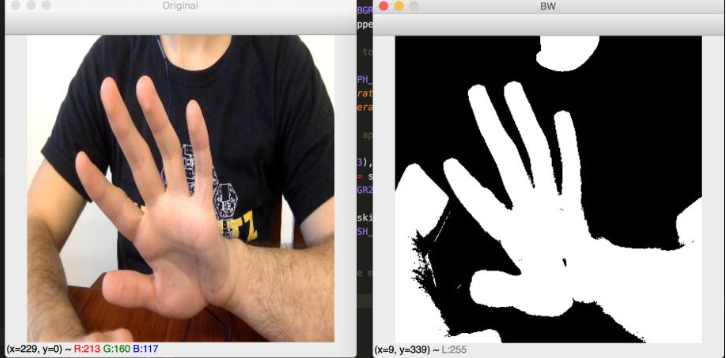
\includegraphics[width=0.5\textwidth]{Haar3.png}
    \caption{ ویژگی های \lr{Haar} برای استفاده از آستانه رنگ پوست برای تشخیص دست}
\end{figure}

این سیستم شامل مراحل پیش‌پردازش داده‌ها، انتخاب ویژگی، ماژول شبکه عصبی برای تشخیص ژست و ماژول کنترل پهپاد برای ترجمه 
ژست‌های شناسایی شده به دستورات حرکت پهپاد می‌باشد. علاوه بر این، از مدل ماشین بردار پشتیبان\LTRfootnote{Support Vector Machine} برای کلاس‌بندی و تشخیص حرکات دست استفاده شده است. ماشین بردار پشتیبان به عنوان یک ماشین یادگیری 
است که برای مسائل دسته‌بندی و رگرسیون استفاده می‌شود و در این پروژه برای تشخیص حرکات دست و ترجمه آنها به دستورات حرکت پهپاد مورد استفاده قرار گرفته است. این روش امکان 
کنترل دقیق و پویا برای پهپاد را فراهم می‌کند و از قابلیت‌های پیشرفته یادگیری عمیق برای تشخیص حرکات دست بهره می‌برد.

\begin{figure}[h]
    \centering
    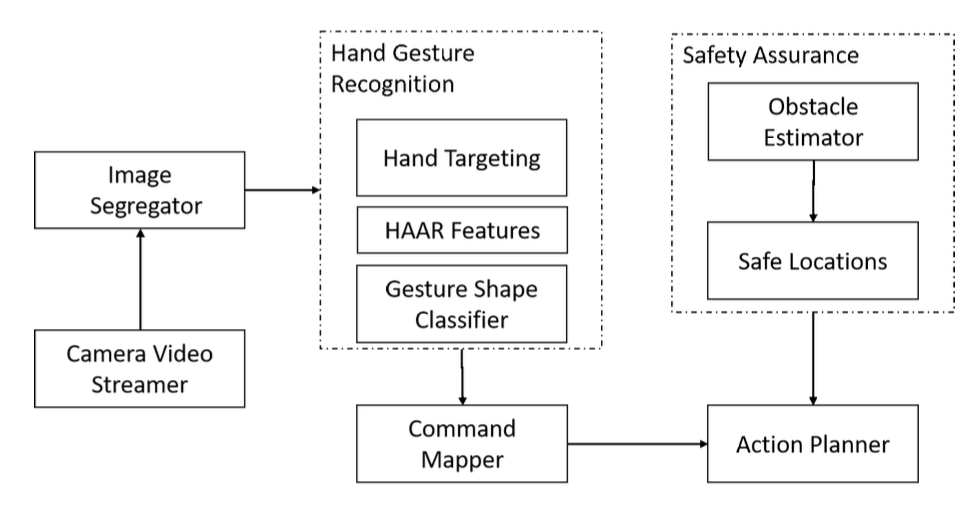
\includegraphics[width=0.8\textwidth]{Haar2.png}
    \caption{چارچوب کنترل پهپاد مبتنی بر ژست دست با کمک ویژگی‌های \lr{Haar}}
\end{figure}

\subsubsection{نتیجه بدست آمده}
این پروژه دقت بالایی در تشخیص ژست دست و کنترل پرواز پهپاد دارد. پنج حالت دست در این پروژه مدنظر قرار گرفته‌اند و دقت متوسط این مدل، برابر ۴۷۱.۹۷ درصد 
است که نشان‌دهنده عملکردی بسیار عالی است. اما لازم به ذکر است که این دقت در پس‌زمینه‌های بهم ریخته و شرایط نوری مختلف 
بسیار متغیر است زیرا ویژگی \lr{Haar} به سایه و رنگ‌های درون تصویر بسیار حساس است.



\subsection{مقاله \lr{A Real-Time Hand Gesture Recognition Method}}
این مقاله در زمینه پردازش تصویر و تشخیص ژست‌های دست، از روش‌های مبتنی بر مدل ظاهری\LTRfootnote{Appearance Model} به عنوان یک رویکرد موثر استفاده کرده‌‌است.
این روش‌ از ویژگی‌های تصویری و حرکتی دست برای تشخیص و تعیین ژست‌های دست استفاده می‌کند. در این مقاله، روش تشخیص ژست‌های دست به صورت زمان واقعی و 
قابل اعتماد است که از تشخیص دست، ردیابی دست\LTRfootnote{Hand Tracking}، تقسیم‌بندی دست\LTRfootnote{Hand Segmentation} و تشخیص ویژگی‌های مقیاس-فضا\LTRfootnote{Scale-Space Feature Detection} برای تشخیص ژست‌ها استفاده می‌کند \cite{fang2007real}.

\subsubsection{روش‌شناسی}
در مقاله از ترکیب متنوعی از روش‌ها و ویژگی‌های تصویری استفاده می‌شود. این ویژگی‌ها به ترتیب به صورت زیر عمل می‌کنند.
\begin{enumerate}
    \item استفاده از روش \lr{Adaboost} برای تشخیص دست، که یک روش معتبر برای تشخیص اشیاء در تصویر است.
    \item پیگیری دست با استفاده از تشخیص حرکت و رنگ، که از ترکیب تکنیک‌های جریان نوری و نشانه رنگ برای ردیابی دست در تصاویر استفاده می‌شود.
    \item تقسیم‌بندی دست با استفاده از اطلاعات حرکت و رنگ برای تمایز دست از پس‌زمینه و اشیاء دیگر. 
    \item تشخیص ویژگی‌های مقیاس-فضا برای تشخیص ژست‌های دست، که برای شناسایی ساختارهای شبیه به کف دست و انگشتان استفاده می‌شود تا نوع ژست دست توسط ترکیب این ساختارها تعیین شود.
\end{enumerate}
  در نهایت این روش‌ها و ویژگی‌ها با هم ترکیب می‌شوند تا یک سیستم تشخیص دست پایدار و دقیق برای استفاده در رابط کاربری تعاملی و تشخیص ژست‌های دست در زمینه‌های مختلف ارائه شود.

\begin{figure}[h]
    \centering
    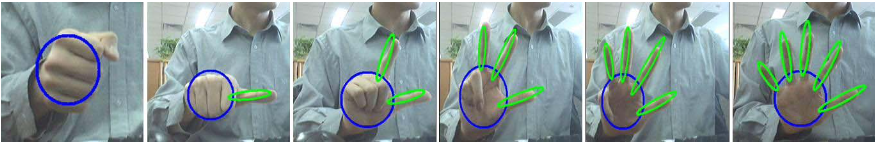
\includegraphics[width=0.8\textwidth]{hand_gesture_feature.png}
    \caption{تشخیص کف دست و انگشتان}
\end{figure}

\subsubsection{نتیجه بدست آمده}
اعمال این روش‌ها نتایج قابل قبولی را به همراه داشته است. دقت مدل در تشخیص ژست‌های دست به صورت میانگین 8.93 درصد بوده و از جمله نتایج مهم آزمایشات می‌توان به تشخیص 
صحیح 2436 فریم از کل 2596 فریم ضبط شده اشاره کرد. این نتایج نشان می‌دهند که روش ارائه شده در این مقاله عملکرد قابل قبولی در تشخیص ژست‌های دست دارد و 
می‌تواند به عنوان یک روش موثر برای تعاملات زمان واقعی استفاده شود.



% \subsection{مقاله \lr{Hand Gesture Recognition using Image Processing and Feature Extraction Techniques}}

% \subsubsection{روش‌شناسی}

% \subsubsection{نتیجه}
% \cite{sharma2020hand}



\section{مقالات مربوط به ورودی تصویر دست به مدل}
مقالات این دسته از جمله پرژه‌هایی هستند که بیشتر از آنکه بر روی پیش پردازش کار کنند باید بر روی معماری خود شبکه تمرکز کنند. در این مقالات تمام یا بخشی از تصویر گرفته شده به صورت یک ماتریس از تصویر با پیکسل‌های متعدد به مدل داده می‌شود. رویکردی که در این نوع پروژه‌ها در پیش گرفته می‌شود، تشخیص موقعیت دست است تا بتوان تنها قسمتی از تصویر را به ورودی شبکه داد که دست در آن وجود دارد تا در حد ممکن
 اندازه ورودی شبکه و دقت آن افزایش یابد. در اینگونه مقالات باید توجه داشت که معماری شبکه را به گونه‌ای برگزید تا در پردازش تصویر بتوان ویژگی‌های تصویر مورد نیاز را استخراج کرد.


\subsection{مقاله \lr{Hand Gestures For Drone Control Using Deep Learning}}
این پروژه نیز با هدف کنترل پهپاد با استفاده از حرکات دست و شبکه‌های عمیق یادگیری انجام شده است تا بتوان ۹ حالت مختلف دست را شناسایی و به پهپاد، دستور موردنظر کاربر را ارسال کرد \cite{hadri2018hand}.

\subsubsection{روش‌شناسی}
در این تحقیق، از معماری شبکه عصبی عمیق \lr{VGG-16} برای تشخیص و تعیین حرکات دست و کنترل پهپاد استفاده شده است. شبکه \lr{VGG-16} یکی از معروف‌ترین و پرکاربردترین شبکه‌های عمیق در زمینه بینایی ماشین است که 
شامل 16 لایه عصبی با لایه‌های کانولوشن و ادغام \LTRfootnote{Pooling} می‌باشد. این شبکه برای استخراج ویژگی‌های مهم از تصاویر استفاده می‌شود. ورودی این شبکه تصاویری است که از دوربین متصل به پهپاد گرفته می‌شود و سپس این 
تصاویر به شبکه وارد می‌شوند. خروجی این شبکه شامل تشخیص حرکات دست مانند حرکات مختلف انگشتان و دست‌ها است. سپس این اطلاعات برای ارسال دستورات کنترلی به پهپاد فرستاده می‌شوند. 

\begin{figure}[h]
    \centering
    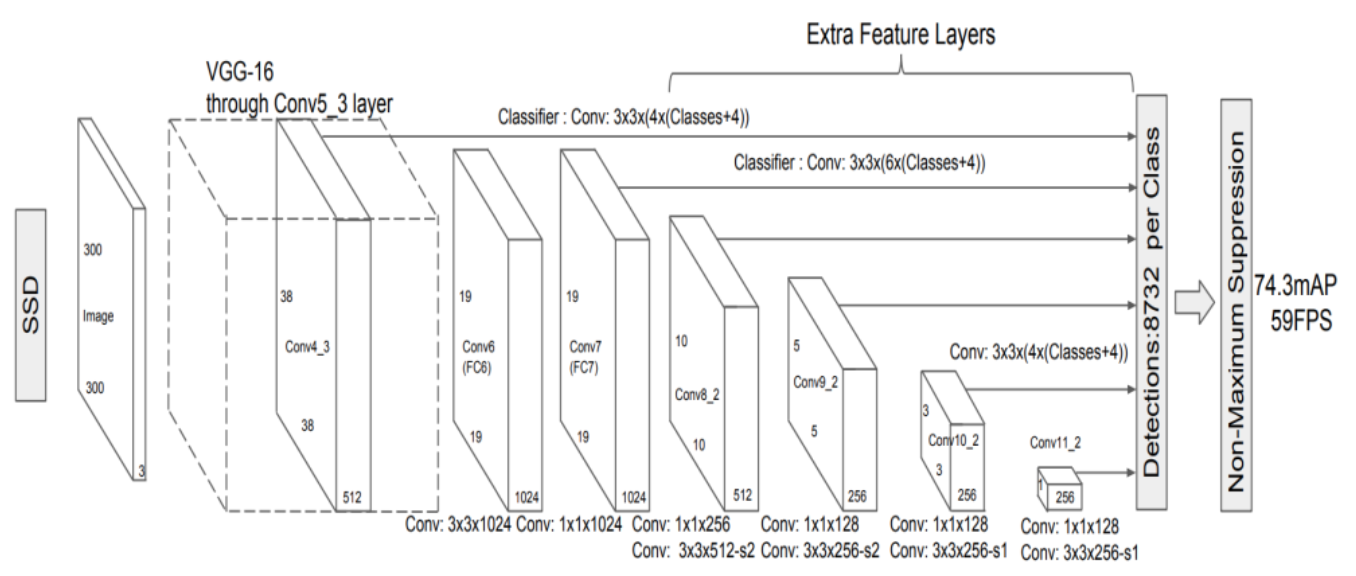
\includegraphics[width=0.8\textwidth]{VGG16.png}
    \caption{معماری \lr{VGG-16}}
\end{figure}

\subsubsection{نتیجه بدست آمده}
 در این پروژه ۹ حالت دست مدنظر قرار گرفته‌شده و دقت آن برابر ۳.۸۳ درصد است.
 که در بهترین حالت ممکن با پس‌زمینه‌ی مناسب بدست آمده و باید در نظر گرفت که دقت بالایی برای کنترل پهپاد به حساب نمی‌آید.


\subsection{مقاله \lr{UAV-GESTURE: A Dataset for UAV Control and Gesture Recognition}}
این مقاله به منظور کنترل پهپاد یا خلبان خودکار با استفاده از حرکت دست پیاده‌سازی شده است. به عنوان مثال، حرکت دست از چپ به راست نشان‌دهنده حرکت پهپاد به راست می‌باشد. 
برای اجرای این برنامه، شبکه \lr{P-CNN} طراحی شده است تا بتواند مفهوم تصاویر را ترجمه کند \cite{perera2018uav}.

\subsubsection{روش‌شناسی}
در این مقاله، از شبکه \lr{P-CNN} \LTRfootnote{Pose-Based Convolutional Neural Network} برای تشخیص حرکات دست استفاده شده است. این شبکه از اطلاعات ژست و حرکت دست و بخش‌هایی از بدن  
استفاده می‌کند. بدین صورت که ابتدا موقعیت دست را با استفاده از جعبه مرزی\LTRfootnote{Bounding Box} مشخص می‌کند و سپس تصویر دست را با استفاده از فیلترهای مناسب وارد شبکه \lr{P-CNN} می‌کند تا بتواند هدف کاربر از حرکت دست را پیش‌بینی کند.
\\
در خروجی این مدل، ۱۳ نوع حرکت مختلف وجود دارد که توسط مدل مفهوم آنها پیش‌بینی می‌شود. این حرکات شامل کل دست از شانه تا انگشتان و حرکات آنها است. این مدل در پروژه برای دستور دادن به هواپیماهای بزرگ بدون سرنشین در فرودگاه‌ها استفاده می‌شود.
\\
\lr{P-CNN} اطلاعات ظاهر و حرکت را از بخش‌های مختلف بدن استخراج و از دو شبکه پیش‌آموزش داده شده برای محاسبه ویژگی‌های \lr{CNN} استفاده می‌کند. در این پروژه برای بخش‌های ژست ظاهری، از شبکه \lr{VGG-f} استفاده می‌شود، و برای 
بخش‌های حرکتی از شبکه \lr{Action Tube} کمک گرفته می‌شود.
در نهایت با ترکیب این دو شبکه با استفاده از روش‌های تجمیع مینیمم و ماکسیمم در هر بعد از تصویر و سپس کنار هم گذاشتن آنها می‌توان حرکت دست را با دقت بالا تشخیص داد.

\subsubsection{نتیجه بدست آمده}
اين مقاله با استفاده از از شبكه \lr{P-CNN} روشي براي كنترل پهپاد با استفاده از حركت و ژست دست پياده‌سازي كرده است. نتايج نشان داده‌اند كه اين روش با دقت ۹.۹۱ درصد، قابليت اجرا در پروژه‌هاي واقعي را دارد.  این پروژه نيازمندي‌هاي پيچيده‌اي براي پياده‌سازي به همراه دارد كه ا بايد در نظر گرفته شود. این شامل نیاز به سخت‌افزار و نرم‌افزار پیشرفته برای پردازش داده‌های حجیم و پیچیده،
 تنظیمات محیطی مانند نورپردازی و شرایط جوی، تنظیمات دقیق برای تشخیص حرکات و ژست‌ها، و مسائل امنیتی مرتبط با کنترل پهپاد است. این چالش‌ها نشان از پیچیدگی‌هایی است که برای اجرای موفق این روش در پروژه‌های واقعی باید در نظر گرفته شوند.




\section{مقالات مربوط به نقاط کلیدی دست}
در این چنین مقالات ورودی شبکه بینایی ماشین برای تشخیص ژست، مختصات نقاط کلیدی دست هستند، که به نوعی یک ویژگی تصویر نیز تلقی می‌شوند. بدین صورت که در ابتدای کار دست کاربرد شناسایی شده و سپس نقاط کلیدی آن استخراج می‌شوند تا بتوان حجم داده ورودی به مدل را تا حد امکان ساده‌تر و در عین حال مفیدتر کرد.

% \subsection{مقاله \lr{Hand Gesture Recognition System for Real-Time Application}}
% این مقاله به بررسی سیستم تشخیص حرکات دست در زمان واقعی می‌پردازد. در این سیستم، از الگوریتم \lr{SIFT} برای استخراج ویژگی‌ها از تصاویر
% حرکتی استفاده شده و سپس از مدل \lr{Bag of Feature} و رده‌بند \lr{SVM} برای تشخیص دقیق حرکات دست و دستیابی به عملکرد زمان واقعی استفاده شده است \cite{murugeswari2014hand}.

\subsection{مقاله \lr{Hand Gesture Recognition System for Real-Time Application}}
این مقاله به بررسی سیستم تشخیص حرکات دست در زمان واقعی می‌پردازد. در این سیستم، از الگوریتم \lr{SIFT} برای استخراج ویژگی‌ها از تصاویر حرکتی استفاده شده است. سپس، از مدل \lr{Bag of Features} و ماشین بردار پشتیبانی برای تشخیص دقیق حرکات دست در زمان واقعی بهره گرفته‌شده‌ است \cite{murugeswari2014hand}.


\subsubsection{روش‌شناسی}
همان‌طور که گفته‌شد در این مقاله از الگوریتم \lr{SIFT} برای استخراج نقاط کلیدی از تصاویر حرکتی دست استفاده شده است. الگوریتم \lr{SIFT} یک الگوریتم معروف برای استخراج ویژگی‌های برجسته 
و تمایزدهنده از تصاویر است که از مقیاس، جهت و از تغییرات نوری برای استخراج این ویژگی‌ها استفاده می‌کند. این ویژگی‌ها به طور قابل توجهی مستقل از 
مقیاس و جهت تصویر هستند و می‌توانند برای کاربرد‌های گوناگونی از جمله، تطبیق قابل اعتماد بین تصاویر مختلف یک شیء مورد استفاده قرار گیرند.

\begin{figure}[h]
    \centering
    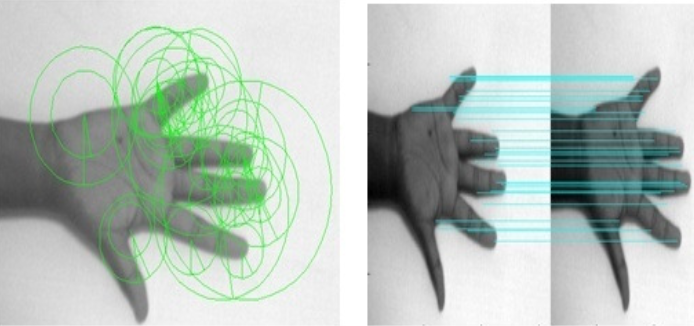
\includegraphics[width=0.5\textwidth]{SIFT.png}
    \caption{تشخیص نقطه کلید و تطبیق توسط \lr{SIFT}}
\end{figure}

\subsubsection{نتیجه بدست آمده}
الگوریتم \lr{SIFT} به عنوان یک ابزار قدرتمند برای استخراج ویژگی‌های برجسته و تمایزدهنده از تصاویر شناخته شده است. این پروژه توانایی تشخیص حرکات دست را با دقت ۸.۹۰ درصد دارد. در این مقاله از روشی نوین و متفاوت برای رسیدن به ژست دست استفاده شده‌است اما قابل ذکر است که این دقت برای پروژه ما می‌تواند خطای زیادی داشته باشد و در روند پروژه استفاده از این الگوریتم کمک‌کننده نیست.




\subsection{مقاله \lr{An Improved Hand Gesture Recognition System Using Keypoints and Hand Bounding Boxes}}
این مقاله یک سیستم بهبود یافته تشخیص حرکات دست با استفاده از نقاط کلیدی و جعبه‌های محدود کننده دست را معرفی می‌کند \cite{dang2022improved}.


\subsubsection{روش‌شناسی}
این پروژه از دو لوله موازی به نام‌های "\lr{MobileNetV2 + FC}" و "\lr{CNN + FC}" تشکیل شده‌است که تصاویر جعبه 
محدود کننده دست و ویژگی‌های استخراج شده از نقاط کلیدی را ترکیب می‌کند و از این طریق ژست دست را پیش‌بینی می‌کند. 
\\
در مدل \lr{MobileNetV2 + FC}، از یک معماری سبک به نام \lr{MobileNetV2} برای استخراج ویژگی‌ها از تصاویر جعبه 
محدود کننده دست استفاده می‌شود. سپس این ویژگی‌ها به یک شبکه عصبی کاملاً متصل (\lr{FC}) داده می‌شوند تا حرکات دست تشخیص داده شوند.
\\
در مدل \lr{CNN + FC} ، در ابتدا نقاط کلیدی دست  که اطلاعات مهمی درباره حرکات دست را شامل می‌شوند پیدا کرده و به یک شبکه عصبی کاملاً متصل وارد می‌شوند تا حرکات دست
تشخیص داده شوند. این مدل از لایه‌های کانولوشنی برای کاهش تعداد پارامترها استفاده می‌کند و سپس از لایه‌های کاملاً متصل برای تشخیص حرکات دست استفاده می‌کند.

\begin{figure}[h]
    \centering
    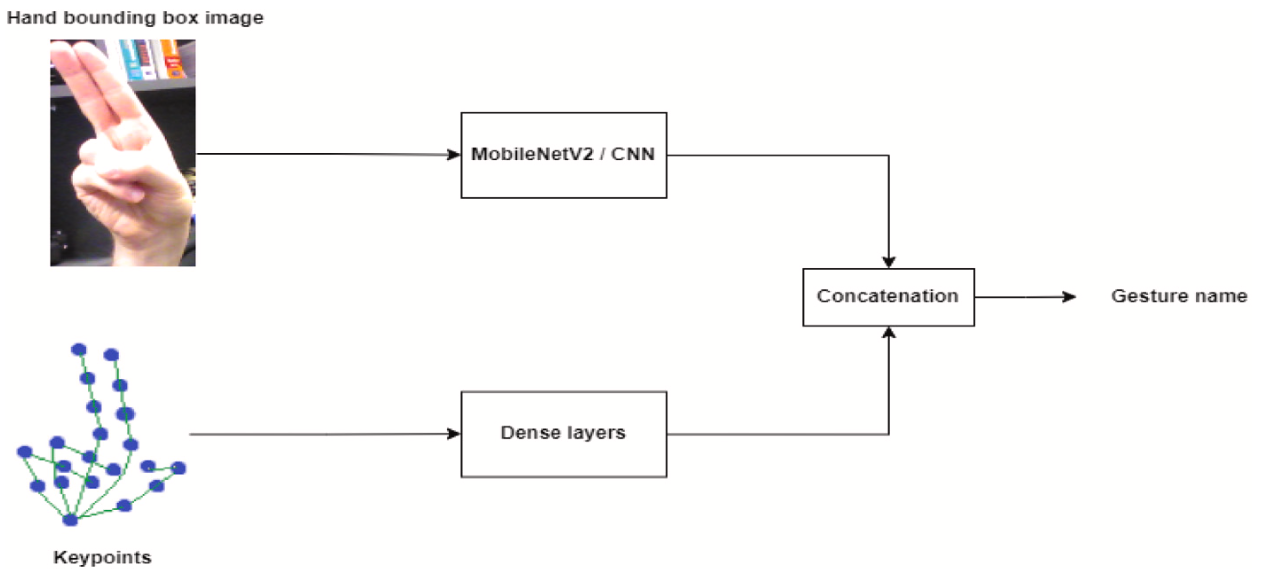
\includegraphics[width=0.8\textwidth]{keypoints_boundingBox.png}
    \caption{معماری ساختار شبکه‌های عصبی دو خط لوله}
\end{figure}


\subsubsection{نتیجه بدست آمده}
در صورتی که دو مدل خروجی‌های متفاوتی را پیش‌بینی کنند، از روش‌های ترکیبی مانند ترکیب احتمالاتی استفاده می‌شود تا بهترین تصمیم برای تشخیص ژست دست گرفته شود.
دقت به دست آمده برای تشخیص ۶ ژست دست مختلف در این مقاله در سه دیتاست متفاوت به ترتیب برابر ۹۱، ۹۴ و ۹۶ درصد است.




\subsection{مقاله \lr{Visual Gesture Recognition Based On Hand Key Points}}
این مقاله یک روش تشخیص حرکات ژستی بصری بر اساس نقاط کلید دست ارائه می‌دهد. این روش ابتدا نقاط کلید دست را در تصویر ورودی فعلی تشخیص می‌دهد و سپس حرکات تعریف شده را تشخیص می‌دهد \cite{chen2021visual}.

\subsubsection{روش‌شناسی}
مدل ارائه شده در این مقاله شامل دو بخش اصلی است: 
\begin{itemize}
    \item مدل تشخیص کف دست که بر اساس ویژگی‌های سخت دست طراحی شده است. برای تشخیص حضور دست در تصویر، از یک مدل \lr{SSD} استفاده شده است که به صورت زمان
    واقعی تشخیص انجام می‌دهد. و نتیجه آن به صورت یک مستطیل نشان داده می‌شود.
    \item    مدل تشخیص نقاط کلیدی دست که پس از تشخیص حضور دست در تصویر، از این مدل برای تشخیص 21 مختصات نقطه کلید سه‌بعدی دست استفاده می‌شود.  این مدل از الگوریتم نرمال‌سازی برای محاسبه مختصات افقی و عمودی هر نقطه 
    دست استفاده می‌کند. یک سیستم مختصات فضایی برای به دست آوردن مختصات عمق هر نقطه دست نسبت به مبدأ مختصات تعیین شده‌است. در نهایت، معنای حرکات در تصویر ورودی بر اساس رابطه مکانی بین مختصات نقاط کلید تعیین می‌شود.
     
\end{itemize}


\begin{figure}[h]
    \centering
    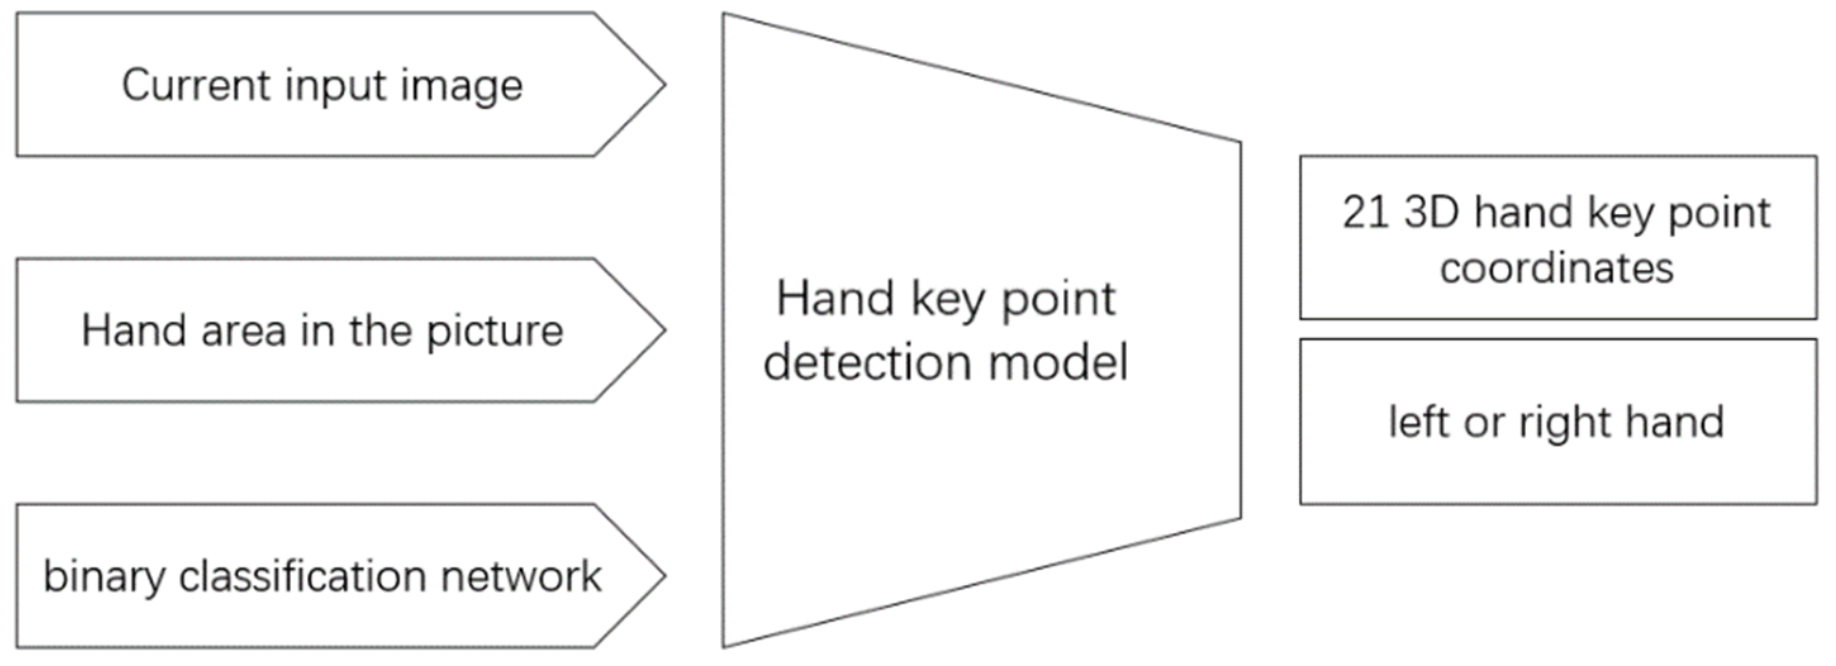
\includegraphics[width=0.7\textwidth]{keypoint.png}
    \caption{ورودی ها و خروجی های مدل تشخیص نقاط کلیدی دست}
\end{figure}

\subsubsection{نتیجه بدست آمده}
این روش دارای دقت بالا و عملکرد مناسبی است. دقت متوسط مدل برابر  ۴.۸۵ درصد تا ۵.۹۸ درصد است که با توجه به جزئیات مدل و پیاده‌سازی پیش‌پردازش می‌تواند انعطاف بالایی داشته باشد در نتیجه می‌تواند راهکار مناسبی تلقی شود.





\subsection{مقاله \lr{MediaPipe Hands: On-Device Real-time Hand Tracking}}
در این مقاله، از کتابخانه \lr{MediaPipe} برای پیش‌بینی ۲۱ نقطه کلیدی دست استفاده‌ ‌شده‌است. این پروژه در موارد گوناگونی از جمله تشخیص ژست دست و افکت‌های واقعیت افزوده \LTRfootnote{Augmented Reality} کاربرد دارد \cite{zhang2020mediapipe}.

\subsubsection{روش‌شناسی}
 برای پیش‌بینی ژست دست  در این پروژه، از دو شبکه کانولوشن استفاده شده‌است. شبکه اول برای پیدا کردن کف دست در تصویر استفاده می‌شود و شبکه دوم ورودی 
موقعیت عکس دست پیدا شده را دریافت و مختصات ۲۱ نقطه عطف را موقعیت‌یابی می‌کند. به کمک این دو شبکه، می‌توان به طور همزمان موقعیت دست‌ها را تشخیص داد و 
نقاط عطف آن‌ها را پیش‌بینی کرد تا برای تشخیص ژست دست در پروژه‌های واقعیت افزوده و واقعیت مجازی استفاده شود.

\subsubsection{نتیجه بدست آمده}
مدل‌های طراحی شده در این مقاله برای تشخیص نقاط عطف دست از دقت ۷.۹۵ درصد برخوردار هستند که دقت بسیار بالایی محاسبه می‌شود. این مدل به نور و تصویر پس‌زمینه 
وابسته نیست و دقت متوسط آن در زمینه‌های مختلف اندازه‌گیری شده، لذا مدل را کاربردی‌تر می‌کند.




\section{مقالات مربوط به آشنایی با پهپاد و اجرای مدل‌های بینایی کامپیوتر روی آن}
% \subsection{مقاله \lr{Modeling Relation Among Implementing AI-Based drones and Sustainable Construction Project Success}}
% این مقاله با بررسی ارتباط بین استفاده از پهپادهای مبتنی بر هوش مصنوعی می‌پردازد. این تحقیق به بررسی تأثیرات مثبتی که ادغام این دو عنصر می‌تواند در بهبود کارایی و پایداری پروژه‌های
% ساختمانی داشته باشد، می‌پردازد. از آنجایی که استفاده از پهپادها در صنعت ساختمان به سرعت در حال افزایش است و شرکت‌های ساختمانی تحت فشار روزافزونی برای اتخاذ 
% تکنیک‌های بیشتر پایدار و کارآمد قرار دارند، شناخت دقیق‌تری از ارتباط بین موانع و عوامل موفقیت لازم است تا بهترین روش‌ها برای از بین بردن موانع و تضمین موفقیت پهپادها در صنعت مشخص شود \cite{waqar2023modeling}.

\subsection{مقاله \lr{Modeling Relation Among Implementing AI-Based Drones and Sustainable Construction Project Success}}

این مقاله به بررسی ارتباط بین استفاده از پهپادهای مبتنی بر هوش مصنوعی و موفقیت پروژه‌های ساخت‌وساز پایدار می‌پردازد. این تحقیق تأثیرات مثبت ادغام
 این دو عنصر را در بهبود کارایی و پایداری پروژه‌های ساختمانی بررسی می‌کند. با توجه به افزایش سریع استفاده از پهپادها در صنعت این مقاله به شناخت دقیقی از ارتباط بین این دو از جمله موانع و موفقیت‌ها می‌پردازد. این شناخت به شناسایی بهترین روش‌ها برای از بین بردن موانع و تضمین موفقیت پهپادها در ترکیب هوش مصنوعی کمک می‌کند \cite{waqar2023modeling}.


\subsubsection{روش‌شناسی}
در این تحقیق، از مدل معادلات ساختاری هوشمند برای بررسی موانع و موفقیت اجرای پهپادهای مبتنی بر هوش مصنوعی در صنعت استفاده شده است.
این مدل شامل یک مجموعه جامع از عوامل موفقیت شامل کیفیت، ایمنی و عوامل محیطی است .
\\
پیاده‌سازی مدل‌ها بر روی پهپادها چالش‌هایی ایجاد می‌کند که باید مورد توجه قرار گیرد. این چالش‌ها شامل موارد زیر می‌شود:
\begin{itemize}
    \item پیچیدگی فنی: پیاده‌سازی مدل‌های هوش مصنوعی بر روی پهپادها نیازمند دانش و تخصص فنی بالا است. این امر نیازمند همکاری بین متخصصان مختلف از حوزه‌های مختلف می‌باشد.
    \item محدودیت‌های سخت‌افزاری: پهپادها ممکن است دارای محدودیت‌های سخت‌افزاری مانند ظرفیت پردازشی و حافظه باشند که ممکن است موانعی برای پیاده‌سازی مدل‌های پیچیده ایجاد کنند.
    \item امنیت و حریم خصوصی: استفاده از هوش مصنوعی در پهپادها نیازمند رعایت استانداردهای امنیتی و حفظ حریم خصوصی است. این امر می‌تواند یک چالش مهم برای پیاده‌سازی مدل‌های هوش مصنوعی باشد.
    \item آموزش و توسعه مدل‌ها: پیاده‌سازی مدل‌های هوش مصنوعی بر روی پهپادها نیازمند آموزش و توسعه مدل‌های مناسب برای محیط و وظایف خاص پهپادها است.
\end{itemize}
این چالش‌ها نشان‌دهنده اهمیت اصلی پیاده‌سازی مدل‌های هوش مصنوعی بر روی پهپادها در صنعت است. با غلبه بر این چالش‌ها، می‌توان بهبود 
قابل توجهی در کارایی، ایمنی و پایداری این گونه پروژه‌‌ها داشت.

\subsubsection{نتیجه بدست آمده}
این مقاله نه تنها به شناخت بهتر موانع استفاده از پهپادهای مبتنی بر هوش مصنوعی کمک می‌کند، بلکه راهکارهایی برای غلبه بر این موانع و افزایش موفقیت این تکنولوژی در صنعت ساختمان ارائه می‌دهد. از آنجا که
پهپادها می‌توانند به صورت خودکار و هوشمند وظایف مختلفی را انجام دهند، این تکنولوژی می‌تواند به بهبود مدیریت پروژه، کاهش هزینه‌ها و زمان اجرا، افزایش کیفیت و ایمنی کارها کمک کند.


\subsection{مقاله \lr{Use of A DJI Tello Drone as An Educational Platform in the Field of Control Engineering}}
این مقاله یک رویکرد نوآورانه را برای استفاده از پهپاد \lr{DJI Tello} به عنوان یک پلتفرم آموزشی در زمینه مهندسی کنترل ارائه می‌دهد. این مقاله به بررسی نحوه استفاده از ویژگی‌های پهپاد برای 
آموزش مفاهیم کنترل به صورت عملی و جذاب و همچنین چگونگی استفاده از پهپاد \lr{DJI Tello} به عنوان یک پلتفرم آموزشی برای مفاهیم کنترل می‌پردازد \cite{ghazi2023use}.

\subsubsection{روش‌شناسی}
در این مقاله، از پهپاد \lr{DJI Tello} به عنوان یک ابزار آموزشی و تحقیقاتی استفاده شده است. این پهپاد به دلیل داشتن حسگرهای متنوع و امکان برنامه‌نویسی با زبان پایتون، به عنوان یک 
ابزار ایده‌آل و انعطاف‌پذیر برای اهداف آموزشی و تحقیقاتی شناخته می‌شود. مقاله به بررسی ارتباط با پهپاد \lr{DJI Tello} از طریق زبان برنامه‌نویسی پایتون، امکانات 
\lr{SDK} رسمی ارائه شده توسط پهپاد، و نحوه ارتباط با پهپاد از طریق وای‌فای و پورت \lr{UDP} می‌پردازد .
\\
در این مقاله، انتخاب پهپاد \lr{DJI Tello} برای نمایش مفاهیم ابتدایی مربوط به حوزه کنترل به دلایل گوناگونی انجام شده‌است. از جمله دلایل انتخاب این پهپاد، محبوبیت رو به افزایش آن در بین عموم مردم،
ویژگی‌های چندگانه آن شامل حسگرها، کنترل بازخورد و الگوریتم‌های تخمین برای انجام وظایف پیچیده، و همچنین قیمت مقرون به صرفه آن نسبت به سایر تجهیزات آموزشی است .
\\
برای پیاده‌سازی مدل‌های هوش مصنوعی بر روی پهپاد \lr{DJI Tello}، از زبان برنامه‌نویسی پایتون و کتابخانه‌های مختلفی که برای ارتباط با حسگرها و سیستم‌های کنترل پروازی پهپاد ارائه شده استفاده می‌شود. این ‌چنین موارداین 
امکان را می‌دهد که مدل‌های هوش مصنوعی توانایی پیاده‌سازی بر روی پهپاد را داشته و عملکرد آن‌ را تحلیل کنند. به عنوان مثال، کاربران می‌توانند از شبکه‌های عصبی یا منطق فازی برای کنترل حرکت پهپاد استفاده کنند.

\begin{figure}[h]
    \centering
    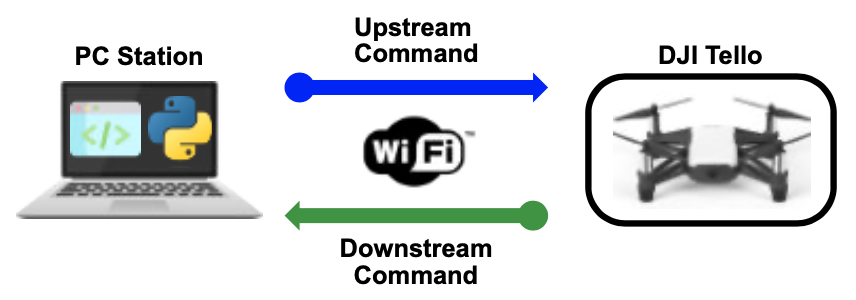
\includegraphics[width=0.8\textwidth]{tello.png}
    \caption{ارتباط برنامه پایتون با پهپاد \lr{DJI Tello}}
\end{figure}

\subsubsection{نتیجه بدست آمده}
نتیجه این مقاله نشان می‌دهد که استفاده از هوش مصنوعی بر روی پهپاد \lr{DJI Tello} به خوبی عمل می‌کند و این ابزار آموزشی و تحقیقاتی می‌تواند به افراد کمک کند تا مفاهیم پیچیده کنترل و هوش مصنوعی را به صورت عملی و جذاب فرا بگیرند. 


\section{جمع‌بندی}

در این فصل به بررسی ۴ گونه مقالات پرداخته‌شد 
\begin{itemize}
    \item مقالاتی که با استفاده از استخراج ویژگی‌های تصویر از جمله نور، جهت، موقعیت و این چنین موارد توانستند ژست دست را تشخیص دهند. این مقالات برای کلاس‌بندی تعداد ژست‌های محدود و گوناگون از یکدیگر به خوبی عمل می‌کنند. در زمانی که تعداد ژست‌ها زیاد شده و حالات دست نزدیک به هم باشند، این دقت به صورت چشم‌گیری کاهش پیدا می‌کند. از آنجایی که تمرکز پروژه ما تعیین ژست دست بدون محدودیت تعداد و حالت است این راهکار به خوبی عمل نمی‌کند.
    \item مقالاتی مربوط به ورودی تصویر دست، نه تنها دقت بالایی از خود نشان نمی‌دهند، بلکه زمان اجرای آنها نسبت به دیگر راهکارها بسیار بیشتر است و می‌تواند پروژه را از زمان واقعی بودن آن که یکی از بزرگ‌ترین اهداف است دور کند.
    \item مقالات مربوط به تعیین ژست دست با استفاده از نقاط کلیدی عملکرد بسیار خوب و دقت بالایی را از خود نشان داد. این مقالات با توجه به اینکه از چندین مدل پی در پی برای تعیین ژست کمک می‌گیرند، اما مدل‌ها حجم پایینی دارند لذا در زمان کوتاهی می‌توان ژست دست را پیش‌بینی کرد. این مقالات راهکار‌های مناسبی را برای کمک پیاده‌سازی پروژه ما ارائه دادند.
    \item مقالات مربوط به آشنایی با پهپاد و اجرای مدل‌های بینایی کامپیوتر روی آن دیدگاه جامعی در مورد پهپاد، مشخصات مورد نیاز آن و چالش‌ها برای اجرای این پروژه به ما نشان دادند.
\end{itemize}

در تمام مقالات بررسي شده، پروژه‌هایی با هدف تعیین ژست دست به گونه‌اي پياده‌سازي شده‌اند تا حركات را به گونه‌ای كلاسبندي كنند كه در خروجي حتما يكي از ژست‌هاي درنظر گرفته‌شده انتخاب شود. لذا زماني كه دست در حالتي غير از آنها قرار دارد، مدل طراحي شده 
حتما يكي از ژست‌هايي را كه به آن شبيه‌تر است انتخاب مي‌كند كه اين امر ميتواند براي پياده‌سازي روي پهپاد واقعي مشكل‌زا باشد و حتي هزينه مالي به ارمغان آورد. برای پیاده‌سازی پروژه ما باید مسیری را در پیش بگیریم تا بتوانیم این مشکل را برطرف کرده و در عین حال دقت بالایی داشته باشیم.